\label{evaluation}



\section{Clustering results}\label{clusteringEvaluation}

\section{Classification results}\label{classificationEvaluation}
\begin{wraptable}[]{l}{0.6\textwidth}
\centering
\scalebox{0.8}{
\begin{tabular}{@{}ll@{}}
\toprule
\rowcolor[HTML]{EEF9FB} 
{\color[HTML]{000000} \textbf{Alias}} & {\color[HTML]{000000} \textbf{Category}} \\ \midrule
\rowcolor[HTML]{DAE8E5} 
{\color[HTML]{000000} C1} & {\color[HTML]{000000} Art} \\
\rowcolor[HTML]{EEF9FB} 
{\color[HTML]{000000} C2} & {\color[HTML]{000000} Deviancy} \\
\rowcolor[HTML]{DAE8E5} 
{\color[HTML]{000000} C3} & {\color[HTML]{000000} Drugs} \\
\rowcolor[HTML]{EEF9FB} 
{\color[HTML]{000000} C4} & {\color[HTML]{000000} Encyklopedia and knowledge} \\
\rowcolor[HTML]{DAE8E5} 
{\color[HTML]{000000} C5} & {\color[HTML]{000000} Fake identity and hitmen} \\
\rowcolor[HTML]{EEF9FB} 
{\color[HTML]{000000} C6} & {\color[HTML]{000000} Finance and Fraud} \\
\rowcolor[HTML]{DAE8E5} 
{\color[HTML]{000000} C7} & {\color[HTML]{000000} Gambling} \\
\rowcolor[HTML]{EEF9FB} 
{\color[HTML]{000000} C8} & {\color[HTML]{000000} Guns} \\
\rowcolor[HTML]{DAE8E5} 
{\color[HTML]{000000} C9} & {\color[HTML]{000000} Hosting, Programming and Hacking} \\
\rowcolor[HTML]{EEF9FB} 
{\color[HTML]{000000} C10} & {\color[HTML]{000000} Online Marketplace} \\
\rowcolor[HTML]{DAE8E5} 
{\color[HTML]{000000} C11} & {\color[HTML]{000000} Other} \\
\rowcolor[HTML]{EEF9FB} 
{\color[HTML]{000000} C12} & {\color[HTML]{000000} Porn} \\
\rowcolor[HTML]{DAE8E5} 
{\color[HTML]{000000} C13} & {\color[HTML]{000000} Social} \\
\rowcolor[HTML]{EEF9FB} 
{\color[HTML]{000000} C14} & {\color[HTML]{000000} Web Catalogue} \\
\rowcolor[HTML]{DAE8E5} 
{\color[HTML]{000000} C15} & {\color[HTML]{000000} Illegal services and goods} \\
\rowcolor[HTML]{EEF9FB} 
{\color[HTML]{000000} C16} & {\color[HTML]{000000} Sexual Content} \\ \bottomrule
\end{tabular}
}
\caption{The alias-category lookup for the Figures in Section \ref{classificationEvaluation}.\label{categoryLegend}}
\end{wraptable}

Four labeled data sets were created as was described in Section \ref{LearningDatasetImplementation}. Ten independent models were trained on each data set. Another ten models were trained with pretrained embeddings on the third samples. The accuracy results of these models are depicted in this section via box plots\footnote{A visual tool for the imaged summarization and comparison of data.} \cite{boxplot}. 

The lower and upper sides of a box in the plot represent the first and the third quartile respectively. The horizontal line inside the box portrays the median. The plus symbol in the box is the mean. The lower and upper whisker ends represent the minimum and maximum values respectively. The name of each box plot corresponds to the utilized training sample data set. Table \ref{categoryLegend} pairs the category shortcuts used in the plots with the actual category names. 

 \begin{figure}[]
    \centering
    \label{CM1Boxplot}
    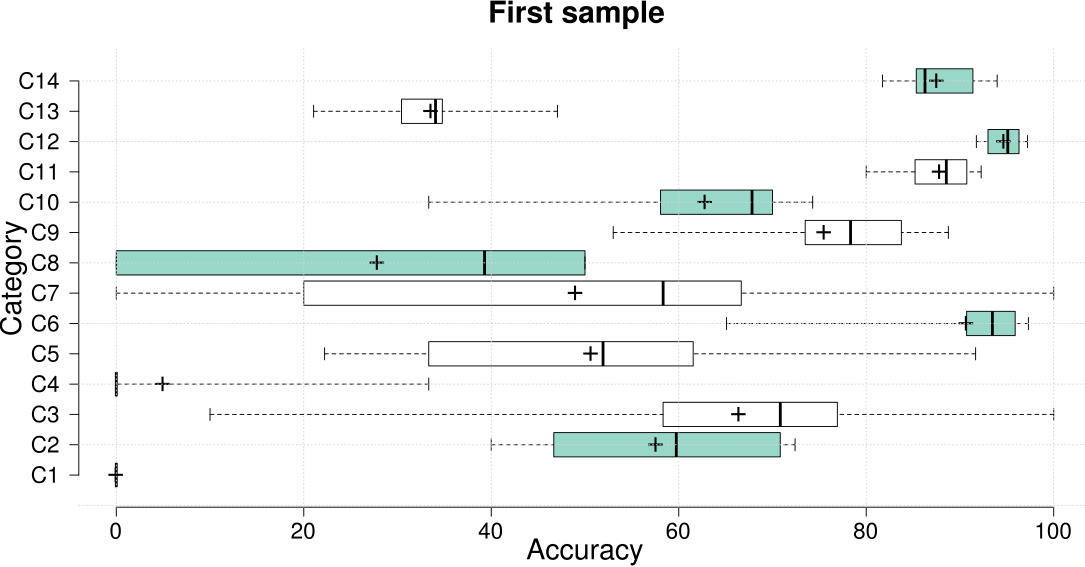
\includegraphics[width =\textwidth]{Images/CM1Boxplot.png}
    \caption{The accuracy per category of the models trained on the first sample. The median of several categories of the first samples were below 70\%. The dispersion was often over 50\%. The individual key values of this plot are detailed in Table \ref{CM1BoxplotValues}.}
    \label{CM1Boxplot}
\end{figure}


 \begin{figure}[]
    \centering
    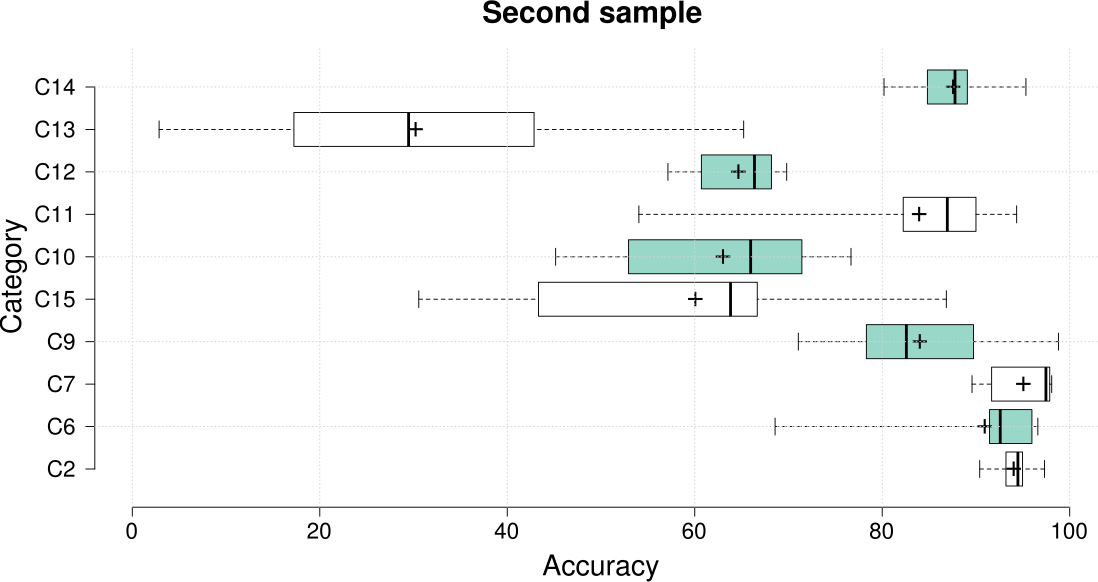
\includegraphics[width =\textwidth]{Images/CM2Boxplot.png}
    \caption{The accuracy per category of the models trained on the second sample. The median of most categories was over 65\%. The dispersion was lowered. The individual key values of this plot are detailed in Table \ref{CM2BoxplotValues}.}
    \label{CM2Boxplot}
\end{figure}

\begin{figure}[]
 \begin{minipage}[t]{\textwidth}
    \centering
    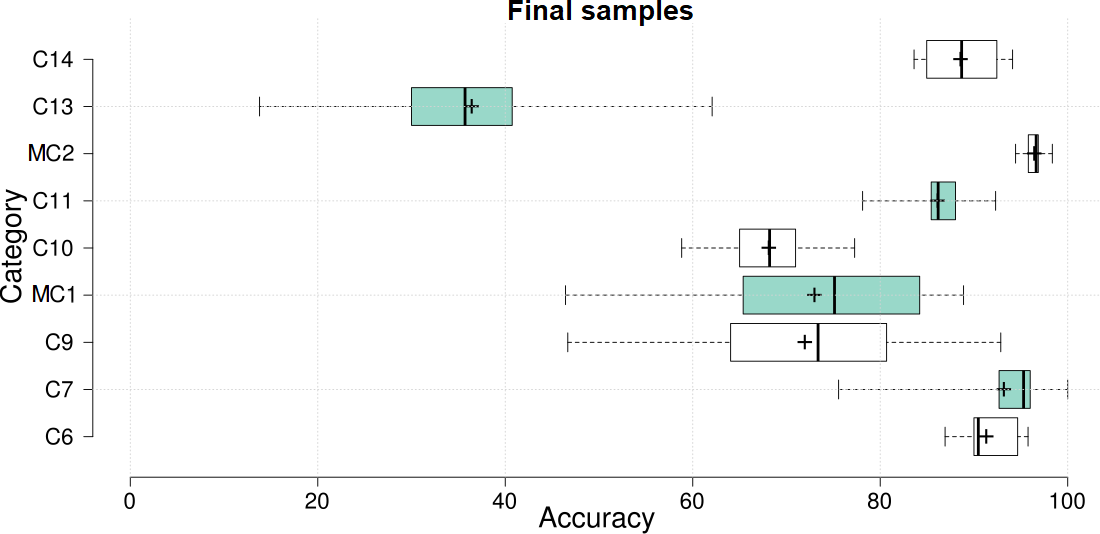
\includegraphics[width =\textwidth]{Images/CM3Boxplot.png}
    \caption{The accuracy per category of the models trained on the third sample. The dispersion was low compared to the results in second samples. The individual key values of this plot are detailed in Table \ref{CM3BoxplotValues}.}
    \label{CM3Boxplot}
\end{minipage}

 \begin{minipage}[b]{\textwidth}
    \centering
    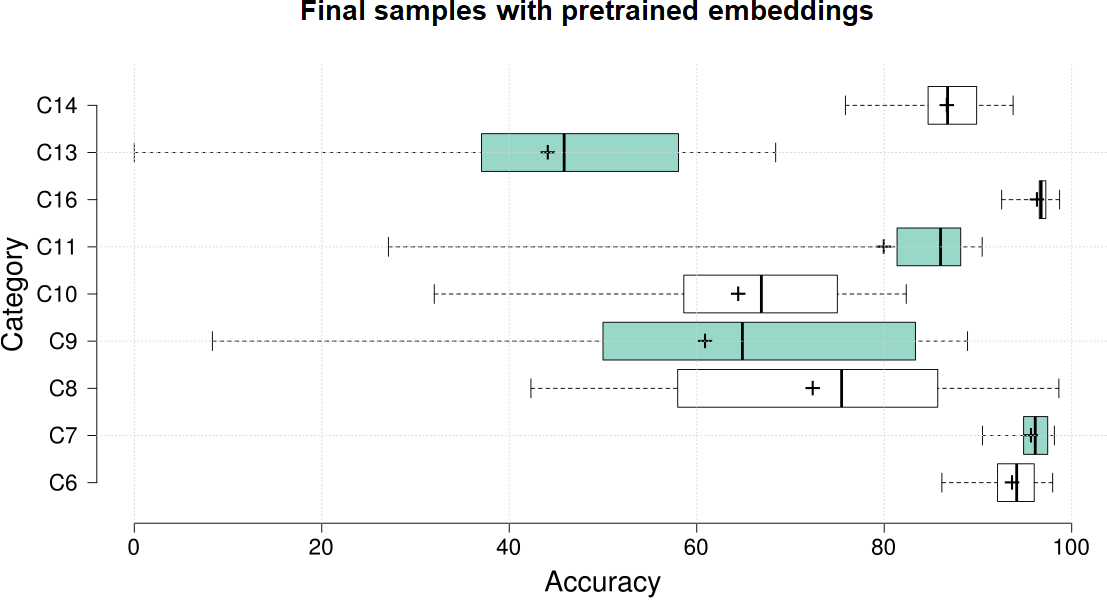
\includegraphics[width =\textwidth]{Images/CM3EmbeddingsBoxplot.png}
    \caption{The accuracy per category of the models trained on the third sample with pretrained embeddings. The maximums and the third quartiles were better compared to the third samples without pretrained embeddings. However, the dispersion of the results was comparatively as bad as in the results with the first sample. The individual key values of this plot are detailed in Table \ref{CM3EmbeddingsBoxplotValues}.}
    \label{CM3EmbeddingsBoxplot}
\end{minipage}
\end{figure} \hfill

 \begin{figure}[t]
    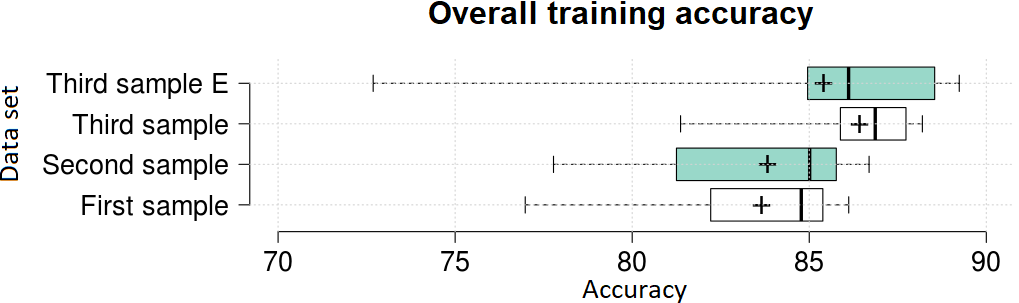
\includegraphics[width =\textwidth]{Images/DSsBoxplot.png}
    \caption{The overall accuracy of the models trained on the dataset samples described in Section \ref{LearningDatasetImplementation}. The data set \textit{Third sample E} stands for the training on the third sample with pretrained embeddings. The individual key values of box plots are detailed in Table \ref{DSsBoxplotValues} }
    \label{DSsBoxplot}
\end{figure}

\FloatBarrier
The learning data set used for the model training was the third sample. The final model utilized in the BE for the categorization of the pages achieved 88.2\% accuracy. We compared these results to two other projects both from the year 2017. The ATOL \cite{atol} classification tool scored an accuracy of 96.4\%. ATOL was used for the categorization of the dark web into 3 categories - drugs, hacker, weapons. The learning data set contained 529 sites. 

The second classifying tool \cite{classificationProject} we compared our results to accomplished an accuracy of 96.6\%. This tool classified the data into 9 categories. The learing approach chosen was SLr. The learning data set contained 6831 pages. 

Both other projects have achieved a higher accuracy. However, ATOL recognized only 3 divergent categories which may explain the high accuracy. The second project adopted a more sophisticated CNN and model balancing. 

